% This file was created with tikzplotlib v0.10.1.
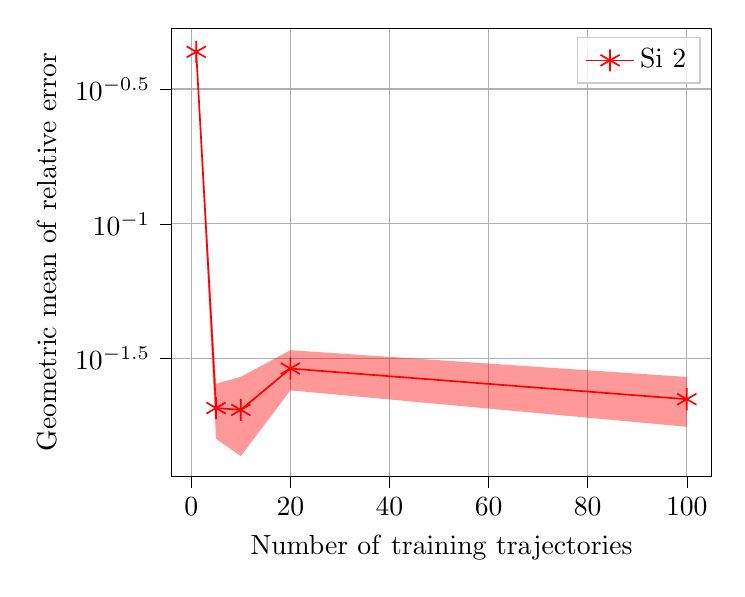
\begin{tikzpicture}

\definecolor{darkgray176}{RGB}{176,176,176}
\definecolor{lightgray204}{RGB}{204,204,204}

\begin{axis}[
legend cell align={left},
legend style={fill opacity=0.8, draw opacity=1, text opacity=1, draw=lightgray204},
log basis y={10},
tick align=outside,
tick pos=left,
x grid style={darkgray176},
xlabel={\(\displaystyle \mathrm{Number \ of \ training \ trajectories }\)},
xmajorgrids,
xmin=-3.95, xmax=104.95,
xtick style={color=black},
y grid style={darkgray176},
ylabel={\(\displaystyle \mathrm{Geometric \ mean \ of \ relative \ error }\)},
ymajorgrids,
ymin=0.0115551905992274, ymax=0.531482631440815,
ymode=log,
ytick style={color=black}
]
\path [fill=red, fill opacity=0.4, semithick]
(axis cs:1,0.446592330072905)
--(axis cs:1,0.421877759191618)
--(axis cs:5,0.0159501810730097)
--(axis cs:10,0.0137516537856237)
--(axis cs:20,0.0241235656092961)
--(axis cs:100,0.0176751562587372)
--(axis cs:100,0.0270518501336542)
--(axis cs:100,0.0270518501336542)
--(axis cs:20,0.0339966001818798)
--(axis cs:10,0.0270795990150381)
--(axis cs:5,0.0255396279098206)
--(axis cs:1,0.446592330072905)
--cycle;

\addplot [semithick, red, mark=asterisk, mark size=4, mark options={solid}]
table {%
1 0.434235036373138
5 0.0207449048757553
10 0.0204156283289194
20 0.029060086235404
100 0.0223635043948889
};
\addlegendentry{Si 2}
\end{axis}

\end{tikzpicture}
